% #############################################################################
% This is Chapter 6
% !TEX root = ../main.tex
% #############################################################################
% Change the Name of the Chapter i the following line
\fancychapter{Evaluation}
\cleardoublepage
% The following line allows to ref this chapter
\label{chapter:evaluation}

\noindent By the end of this project we've successfully implemented a framework that enables developers to use an agency model, \ac{FAtiMA}, to create \acp{NPC} for Don't Starve Together.
This was achieved through the implementation of a modification for \ac{DST} and a companion console application.
As contributions resultant from this work we also count with a tutorial for creating \acp{NPC} and an example \ac{NPC}.

For the remainder of this chapter we will talk about the published \textit{mod}, then we will talk about a use case of the framework, and will finish with a comparison between our example character and the work of an anonymous developer.

\section{Walter - The AI Companion}

\noindent As said before, the example character we created to demonstrate the framework has been published in the Steam Workshop.
At the time of writing, with 48 days of existence, the \textit{mod} counts with 738 unique viewers and 128 subscribers, as shown in Figure \ref{fig:walter-stats}.

While subscribers represent the number of people who've added the \textit{mod} to their game, it does not tells us how many of those have actually used the \textit{mod}.
The \textit{mod} also counts with 25 comments on the public page, mostly related to running the mod.

Although it has received no direct negative feedback, we believe that the necessity of running a separate console application has greatly impacted the community's acceptance and use of the \textit{mod}.
Additionally, to the best of our knowledge, no member of the community has used our framework to develop their own \acp{NPC}.

\begin{figure}
  \centering
  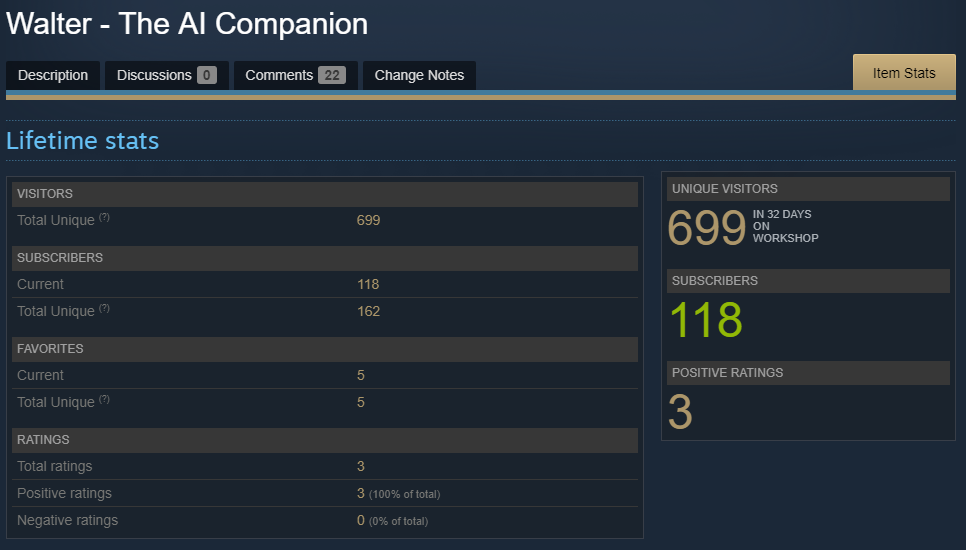
\includegraphics[width=\textwidth]{./Images/walter-stats}
  \caption{Walter - The AI Companion \textit{mod} lifetime stats.}
  \label{fig:walter-stats}
\end{figure}

\section{Monte Carlo Tree Search Project}

\noindent As part of the Artificial Intelligence for Games course taught at Instituto Superior Técnico, a group of three students used our framework for their final project.
The project consisted in the implementation of the \ac{MCTS} algorithm for the decision process of the agent.

Briefly, the \ac{MCTS} algorithm is based in a random exploration of a state space.
By randomly (and rapidly) collecting data of the space state, the algorithm will gradually improve its knowledge of what the best next move is.

Unlike many other algorithms, \ac{MCTS} does not run until an answer is found.
Instead, the usual approach consists in letting the algorithm run for some time (or a certain number of iterations) and then return the best possible action, in regard to the information collected so far.
The algorithm has proven to be especially good in problems where the space state has an high branching factor and many possible combinations, such as the Go game.

In this case, the implementation of the \ac{MCTS} algorithm was achieved through the use of \ac{FAtiMA}'s Dynamic Properties.
The created Dynamic Property, called \texttt{MCTS}, will use current knowledge base and apply the \ac{MCTS} algorithm.
The \ac{MCTS} algorithm was let run for two thousand iterations (about twenty seconds) before returning a plan to act upon.

One of the main difficulties found during this use case was related to the random exploration of the state space.
As Don't Starve Together does not provide a way to simulate the resulting state of applying actions and \ac{FAtiMA} did not have such functionality either (although it can now achieve this through the use of the World Model Asset), the group had to create their own simulator of the Don't Starve Together world.

This work, praises the versatility of our framework by demonstrating the ability to create a planning agent based on \ac{MCTS}.
Although the group had to struggle with the world simulation, the end result was an \ac{NPC} for \ac{DST} with planning capabilities.

\section{Walter vs. Artificial Wilson}

\noindent As a means of evaluating the created \ac{NPC}, we've run it and recorded how long it can survive.
Additionally, we compare it to an unpublished character for Don't Starve, Artificial Wilson.

Artificial Wilson, is the work of the anonymous \textit{modder} KingofTown and can be found in the public repository \href{https://github.com/KingofTown/DS-AI}{https://github.com/KingofTown/DS-AI}.

\subsection{Testing Conditions}

\noindent For each run of the characters, a new world was dynamically generated with equal sets of constraints for both characters.
The characters were then let run for as long as possible until their death.

As we said, Artificial Wilson was created for the original game, Don't Starve.
Therefore it is incompatible with Don't Starve Together because of the updates made to turn it into a multiplayer game.
However, the game mechanics and configurations remain the same.

As such, we can use the scenario configurator to generate equivalent worlds.
For this test, we considered the following restrains:

\begin{itemize}
	 \item \textbf{A world with no enemies}: all aggressive monsters have been removed from the game as well as the giants.
     \item \textbf{No random meteorological events}: apart from raining all other events have been disabled (like meteors,  frog rains, lightning storms, and wildfires).
     \item \textbf{No resurrection stones}: if the \ac{NPC} dies, it stays dead.
     \item \textbf{No matting season for \textit{beefalos}}: during this season these, normally pacific creatures, will attack any character on sight.
     \item \textbf{No modifications}: apart from the necessary ones for running both characters.
     \item \textbf{Only one \ac{NPC} and no players}: while in Don't Starve this does not apply, in Don't Starve Together the tests were run locally with no players present in the world.
\end{itemize}

These constrains will generate similar worlds for both Don't Starve and Don't Stave Together.
For each play-through of an agent, a new world is generated with these sets of constraints.
Each generated world is unique but complies to the specified set of constraints.

\subsection{The Results}

\noindent Each character has been run thirty times and the survival duration for each character is presented in Figures \ref{fig:days-survived-walter} and \ref{fig:days-survived-wilson}.

\begin{figure}
  \centering
  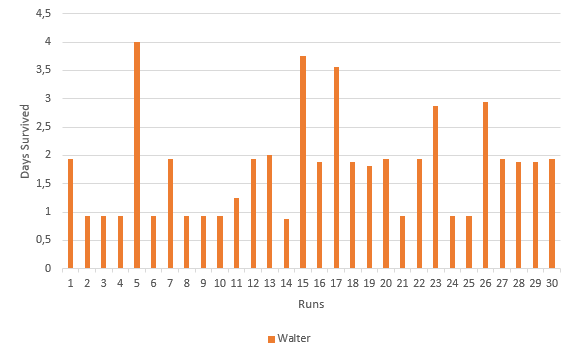
\includegraphics[width=\textwidth]{./Images/days-survived-walter}
  \caption{Days survived for Walter.}
  \label{fig:days-survived-walter}
\end{figure}

\begin{figure}
  \centering
  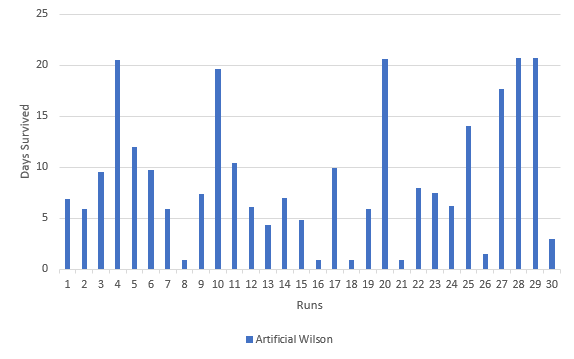
\includegraphics[width=\textwidth]{./Images/days-survived-wilson}
  \caption{Days survived for Artificial Wilson.}
  \label{fig:days-survived-wilson}
\end{figure}

\begin{figure}
  \centering
  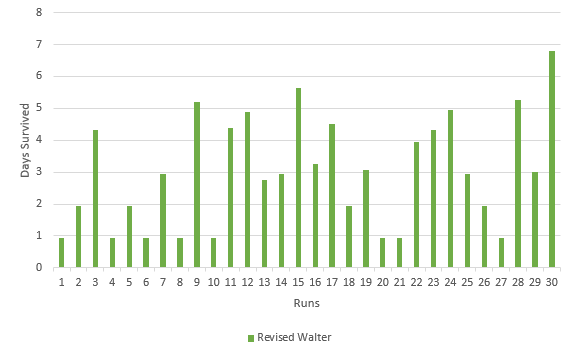
\includegraphics[width=\textwidth]{./Images/days-survived-walter-new-and-improved}
  \caption{Days survived for revised version of Walter.}
  \label{fig:days-survived-walter-new-and-improved}
\end{figure}

Walter survived, on average, one point eight days while Artificial Wilson survived, on average, eight point nine days.
The percentage difference of 132\% between both values can be explained by the detail put in each character's decision process\footnote{Percentage difference equals the absolute value of the change in value, divided by the average of the 2 numbers, all multiplied by 100. We then append the percent sign, \%, to designate the \% difference.}.

Walter is a model based agent with nineteen rules of decision.
Each of these rules has no decision process besides the character's ability to perform it (e.g. does the \ac{NPC} has an axe equipped to cut down a tree?, does it have the required ingredients to build a fire?).

Artifical Wilson is based on the built-in behaviour trees.
The final behaviour tree counts with over seventy nodes and dozens of helper functions.
Embedded in the \acp{NPC}'s decision process are some planning capabilities and resource management (e.g. the \ac{NPC} will ignore resources if she has already gathered enough of it), which Walter does not possess.

If we compare both characters to real human players, Walter has the ability of a newcomer who as never played the game, while Artificial Wilson could be compared to a returning player who played the game for a couple dozen of times\footnote{This comparison has been based on the writer's experience with the game}.

For each character we've recorded not only their survival time but also their cause of death.
In Table \ref{tab:cod} you can see a summary for both characters.

\begin{table}[htb]
	\centering
    \caption{Artificial Wilson, Walter, and Revised Walter cause of death summary.}
    \label{tab:cod}
    \begin{tabular}{ | p{0.18\linewidth} | p{0.1\linewidth} | p{0.18\linewidth} | p{0.1\linewidth} | p{0.18\linewidth} | p{0.1\linewidth} |}
        \hline 
        \multicolumn{2}{|c|}{Artificial Wilson} & \multicolumn{2}{|c|}{Walter} & \multicolumn{2}{|c|}{Revised Walter} \\ \hline 
        Cause of Death & Times & Cause of Death & Times & Cause of Death & Times \\ \hline
        Cactus & 2 & Darkness & 18 & Darkness & 17 \\ \hline
        Cold & 5 & Fire & 8 & Hunger & 13 \\ \hline
        Darkness & 10 & Hunger & 4 & & \\ \hline
        Hunger & 13 & & & & \\ \hline
    \end{tabular}
\end{table}

We can see that Walter died several times due to fire damage.
Upon analyzing its behaviour, we observed that this was due to the \ac{NPC}'s placement of campfires.
The reactive rules we've empowered Walter with, have no concern for the placement of structures.
As such, the \ac{NPC} would often build campfires in the middle of forests that would be set ablaze by the campfire. This, in turn, would cause the \ac{NPC} to die by fire.

In order to counteract this, we decided to disable the rule for building campfires.
Instead the agent relies on torches to illuminate itself through the night.
The results are presented in Figure \ref{fig:days-survived-walter-new-and-improved}.
The average surviving time for Walter increased from one point eight days to three days, which represents an increase of 66\%. 

%The problem with the placing of structures as also been considered for future work.
%An helper function that finds a suitable place for construction, near the position specified by the \ac{AI} would solve this and future problems related to structure placement.

\subsection{Notes on Character Behaviour}

\noindent We would like to note some aspects we found interesting from both character's behaviour.

While Artificial Wilson has a selective picking and manages his inventory, Walter's reactive behaviour lacks this features.
In fact, for runs that Walter was able to survive more that two, three days it became apparent that the lack of space in the inventory was a great hindrance.
Most of the time Walter would collect many items that would just occupy space in the inventory without ever using them.

Regarding the map exploration, Artificial Wilson would end up by exploring a lot more of the map than Walter.
This is directly related to the point discussed before.
By picking only what it needs, Artificial Wilson would move on to unexplored territories to find what it needed.
On the other hand, Walter would stay around the same place for extensive amounts of time.

This brings us to the third aspect we would like to discuss.
By staying on the same area, Walter would eventually deplete all the available resources.
This killed him most of the time, due to the lack of food or materials to make a torch for the night.
Artificial Wilson however, did not suffer from this problem as it roamed the world more extensively, being able to recollect certain resources that would regrow while it was exploring other parts of the world.
By comparison, Walter's decision making is too heavily focused on exploiting its available resources and providing a better exploration-exploitation balance could lead to better results.
